\excercise{Mehr Shapes}

\begin{enumerate}
	\item
	Passe die Main Operation an die Aufgabe an.\\
	Verwende \lstinline{Sheet4Task3}, auch in dieser Aufgabe gibt es keinen Verifier.
	
	\item
	Überlege dir neue Shapes (Formen) und implementiere diese.
	Als Beispiel könntest du eine neue Form erstellen, welche dir ein ausgefülltes Rechteck oder eine Diagonale zeichnet.
	Natürlich ist der Kreativität hier keine Grenze gesetzt.
	
	\textbf{Tipp:} Es gibt bereits Shapes die wir im Paket \lstinline{de.unistuttgart.informatik.fius.jvk.provided.shapes} erstellt haben.
	
	\item
	Nun da wir Shapes etwas genauer kennengelernt haben, können wir damit Spielfelder frei bauen.
	Erstelle ein Labyrinth aus Büschen.
	\optional{Überlege dir wo der Start und das Ende des Labyrinths ist und löse es mit der Spielfigur.}
	
	\item
	\optional{Versuche das folgende Spielfeld im Code nachzubauen.}\\
		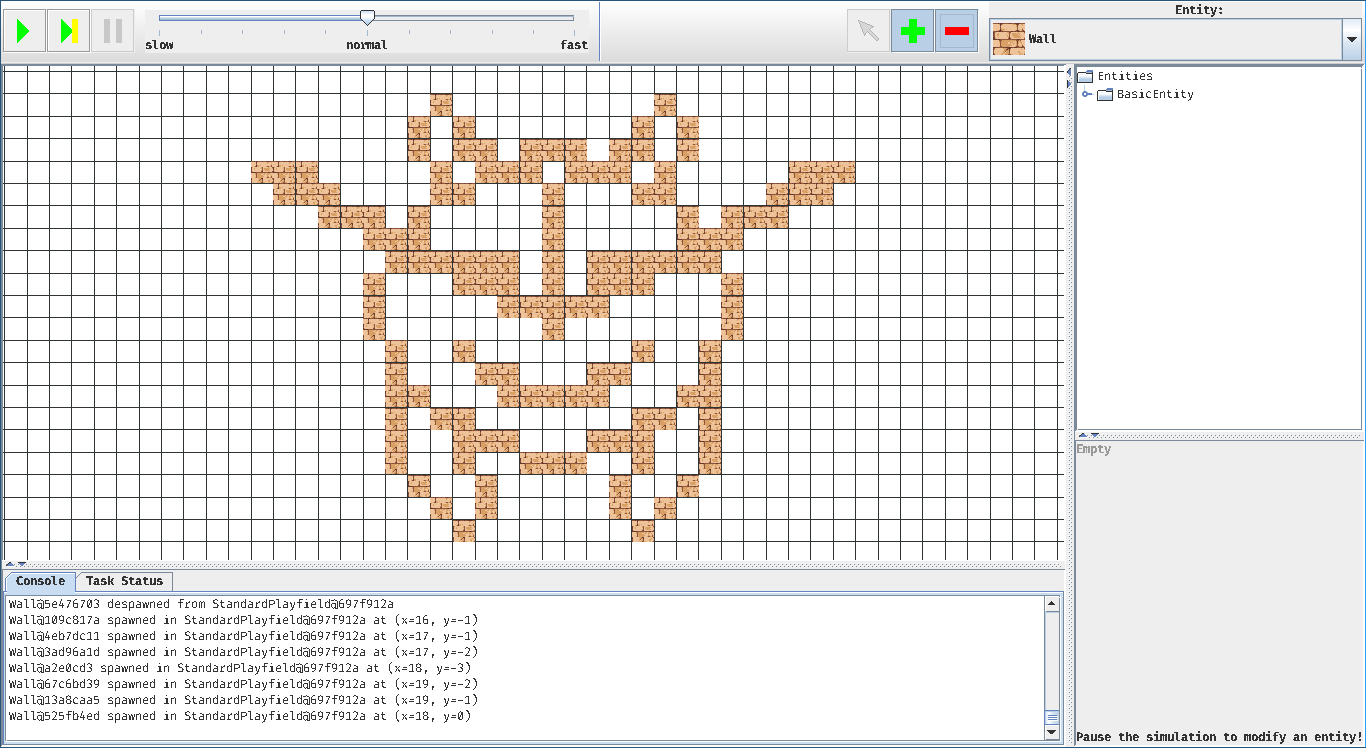
\includegraphics[width=\linewidth]{./figures/playfield.png}

\end{enumerate}

\newpage
